%天体运动的简单数值计算

\pentry{万有引力\upref{Gravty}, 弹簧振子受迫运动的简单数值计算\upref{SHOFN}}

直角坐标系中, 设中心天体质量为 $M$, 固定在原点不动.根据牛顿万有引力定律,质量为 $m$ 的行星受到中心天体的力为
\begin{equation}
\vec F = -G \frac{Mm}{r^2}\uvec r = -G\frac{Mm}{r^3} \vec r
\end{equation}
其中 $\vec r$ 为行星的位矢(设行星在 $xy$ 平面上运动). 根据牛顿第二定律\upref{New3}, 加速度为
\begin{equation}
\vec a = \frac{\vec F}{m} = -G\frac{M}{r^3} \vec r
\end{equation}
用 $r = \sqrt{x^2+y^2}$ 以及 $\vec r = x\uvec x + y\uvec y$, 其中 $x,y$ 看成 $t$ 的函数. 考虑到 $a_x = \dv*[2]{x}{t}$, $a_y = \dv*[2]{y}{t}$, 可以列出二阶微分方程组
\begin{equation}\label{KPNum0_eq3}
\leftgroup{
\dv[2]{x}{t} = -\frac{GM}{(x^2+y^2)^{3/2}}x\\
\dv[2]{y}{t} = -\frac{GM}{(x^2+y^2)^{3/2}}y
}\end{equation}
假设已知初值条件 $x(0) = x_0$, $y(0) = y_0$, $\dot x(0) = v_{x0}$, $\dot y(0) = v_{y0}$. 下面用“弹簧振子受迫振动的简单数值计算\upref{SHOFN}” 中类似的方法求接下来行星的运动轨迹.

1.将初始条件代入\autoref{KPNum0_eq3},得到初始加速度
\begin{equation}
\leftgroup{
\ddot x(0) &= -\frac{GM}{(x_0^2 + y_0^2)^{3/2}} x_0\\
\ddot y(0) &= -\frac{GM}{(x_0^2 + y_0^2)^{3/2}} y_0
}
\end{equation}
 
2.设经过一段极微小的时间步长 $\Delta t$ (例如 $0.0001$, 数值越小误差越小), 根据微分近似(微分近似在这里的物理意义是在 $\Delta t$ 内速度和加速度都近似为常数)
\begin{equation}
\leftgroup{
\dot x(\Delta t) &\approx \ddot x(0)\Delta t + x(0)\\
\dot y(\Delta t) &\approx \ddot y(0)\Delta t + \dot y(0)}
\qquad
\leftgroup{
x(\Delta t) &\approx \dot x(0)\Delta t + x(0)\\
y(\Delta t) &\approx \dot y(0)\Delta t + y(0)}
\end{equation}

3.把 $x(\Delta t), y(\Delta t)$ 再次代入\autoref{KPNum0_eq3}, 得到 $x''(\Delta t), y''(\Delta t)$, 再次利用微分近似求出 $x(2\Delta t), y(2\Delta t), x'(2\Delta t), y'(2\Delta t) \dots$ 如此循环下去就可以得到每隔 $\Delta t$ 的数值解.

\Code{kepler}

程序运行结果如\autoref{KPNum0_fig1} 所示. 注意行星轨道并不是一个闭合的椭圆, 这是由于这种算法误差较大, 为了减小误差, 可以增加程序中\x{Nstep}的值.
\begin{figure}[ht]
\centering
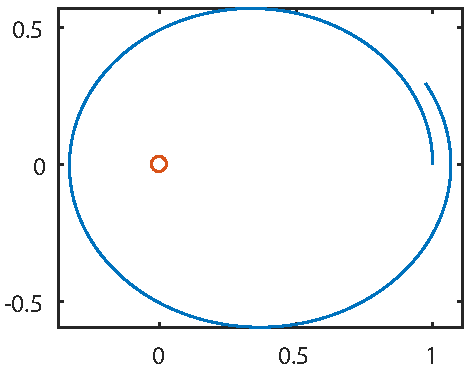
\includegraphics[width=7cm]{./figures/KPNum01.pdf}
\caption{运行结果} \label{KPNum0_fig1}
\end{figure}
